\newpage
\begin{figure}[hbt!]
\chapter{程式}
\section{程式講解}
\end{figure}
1.先用xml製作記分板,然後用sim.getObjectPosition將bubbleRob、bubbleRob2和球的初始位置紀錄下來,然後用sim.getObjectOrientation將初始方向記錄下來。
\begin{center}
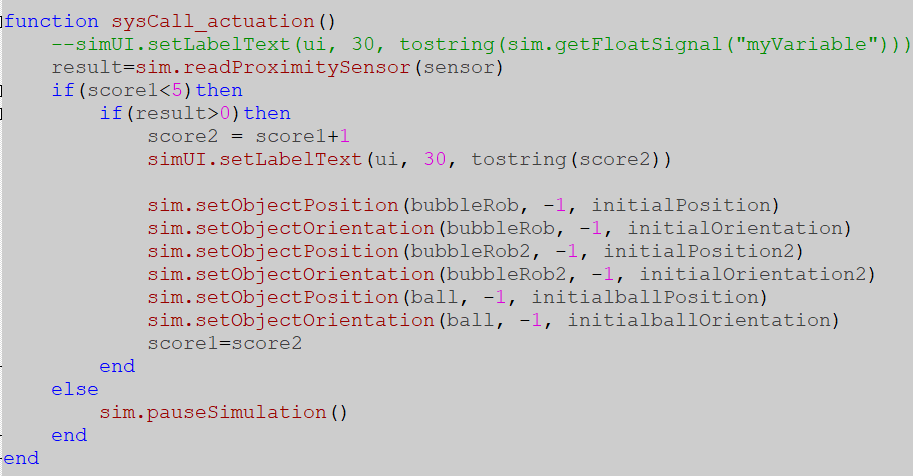
\includegraphics[angle=0,width=12cm]{48.4}
\end{center}

2.sim.readProximitySensor這個函數若傳感器未檢測到任何物體,返回值將是負數。如果傳感器與一個物體相交,返回值將是一個非負數的距離值,所以可以用if迴圈判斷函示返回值大於零去做加分跟回歸初始位置的動作
simUI.setLabelText(ui, 30, tostring(score2))這個函式則是將獲地的分數轉成string並輸入到id為30的text。
\begin{center}
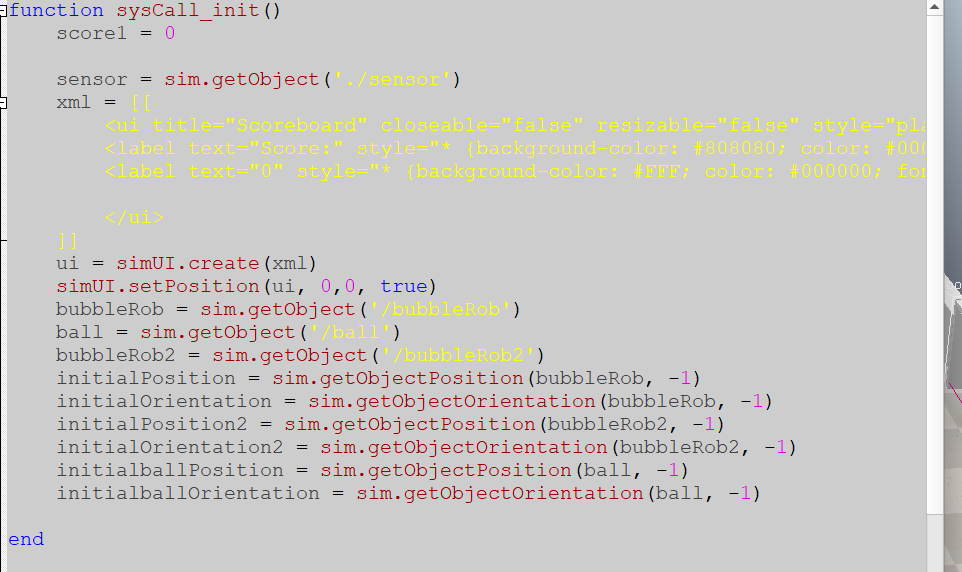
\includegraphics[angle=0,width=12cm]{48.6}
\end{center}
\newpage
3.這個程式要執行要先下載兩個東西pip install keyboard、pip install pyzmq cbor將這兩行打進cmd執行。
\begin{center}
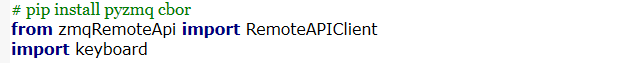
\includegraphics[angle=0,width=15cm]{48.7}
\end{center}

4.這個程式要連線遠端電腦要將:\\
client=RemoteAPIClient('localhost', 23000)\\
中的localhost改成遠端電腦的ipv4位址並將遠端電腦的防火牆關掉,後面只要這個軸('/leftMotor')('/rightMotor')的名稱對應到coppeliasim就可以遠端控制。
\begin{center}
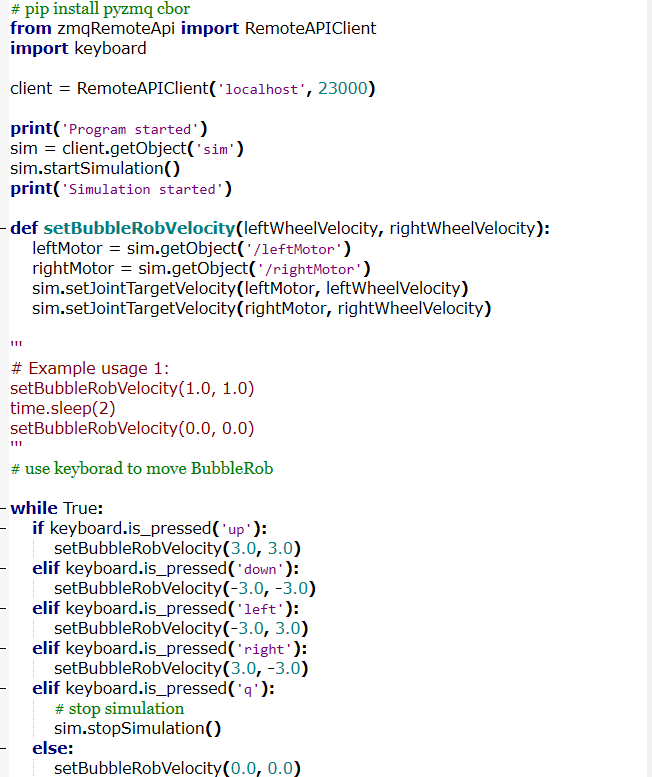
\includegraphics[angle=0,width=14cm]{48.8}
\end{center}